\section{JavaScript}

% Console and Data Types
\begin{formula}{Web-Konsole}
    JavaScript Console im Browser:
    \begin{itemize}
        \item \texttt{console.log(message)}: Gibt eine Nachricht aus
        \item \texttt{console.clear()}: Löscht die Konsole
        \item \texttt{console.trace(message)}: Stack trace ausgeben
        \item \texttt{console.error(message)}: stderr ausgeben
        \item \texttt{console.time()}: Timer starten
        \item \texttt{console.timeEnd()}: Timer stoppen
    \end{itemize}
    API-Dokumentation: \url{https://nodejs.org/api/console.html}
\end{formula}

\begin{definition}{Datentypen}
    JavaScript kennt folgende primitive Datentypen:
    \begin{itemize}
        \item \texttt{number}: 64-Bit Floating Point (IEEE 754)
        \begin{itemize}
            \item \texttt{Infinity}: $1/0$
            \item \texttt{NaN}: Not a Number ($0/0$)
        \end{itemize}
        \item \texttt{bigint}: Ganzzahlen beliebiger Größe (mit n am Ende)
        \item \texttt{string}: Zeichenketten in \texttt{''}, \texttt{""} oder \texttt{``}
        \item \texttt{boolean}: \texttt{true} oder \texttt{false}
        \item \texttt{undefined}: Variable deklariert aber nicht initialisiert
        \item \texttt{null}: Variable bewusst ohne Wert
        \item \texttt{symbol}: Eindeutiger Identifier
    \end{itemize}
\end{definition}

\begin{KR}{typeof-Operator}\\
Mit \texttt{typeof} kann der Typ eines Wertes ermittelt werden:
\begin{lstlisting}[language=JavaScript, style=basesmol]
typeof 42          // 'number'
typeof 42n         // 'bigint'
typeof "text"      // 'string'
typeof true        // 'boolean'
typeof undefined   // 'undefined'
typeof null        // 'object' (!)
typeof {}          // 'object'
typeof []          // 'object'
typeof (() => {})  // 'function'
typeof Infinity    // 'number'
typeof NaN         // 'number' !!
typeof 'number'    // 'string'
\end{lstlisting}
\end{KR}

\begin{theorem}{Variablenbindung}\\
    JavaScript kennt drei Arten der Variablendeklaration:
    \begin{itemize}
        \item \texttt{var}
        \begin{itemize}
            \item Scope: Funktions-Scope (Global oder Lokal)
            \item Eigenschaften: Kann neu deklariert werden
        \end{itemize}
        \item \texttt{let}
        \begin{itemize}
            \item Scope: Block-Scope (innerhalb von \{\})
            \item Eigenschaften: Moderne Variante für veränderliche Werte
        \end{itemize}
        \item \texttt{const}
        \begin{itemize}
            \item Scope: Block-Scope (innerhalb von \{\})
            \item Eigenschaften: Wert kann nicht neu zugewiesen werden
        \end{itemize}
    \end{itemize}
\end{theorem}

\begin{corollary}{Operatoren}
    \begin{itemize}
        \item Arithmetische Operatoren: $+, -, *, /, \%, ++, --$
        \item Zuweisungsoperatoren: $=, +=, -=, *=, /=, \%=, **=, $\\$<<=, >>=, >>>=, \&=, ^=, |=$
        \item Vergleichsoperatoren: $==, ===, !=, !==, >, <, >=, <=$
        \item Logische Operatoren: $\&\&, ||, !$
        \item Bitweise Operatoren: $\&, |, ^, ~, <<, >>, >>>$
        \item Sonstige Operatoren: \texttt{typeof}, \texttt{instanceof}
    \end{itemize}
\end{corollary}

\begin{formula}{Vergleichsoperatoren}
    JavaScript unterscheidet zwei Arten von Gleichheit:
    \begin{itemize}
        \item \texttt{==} und \texttt{!=}: Mit Typumwandlung
        \item \texttt{===} und \texttt{!==}: Ohne Typumwandlung (strikt)
    \end{itemize}
\begin{lstlisting}[language=JavaScript, style=basesmol]
5 == "5"     // true  (Typumwandlung)
5 === "5"    // false (keine Typumwandlung)
null == undefined    // true
null === undefined   // false
\end{lstlisting}
\end{formula}

\begin{KR}{Verzweigungen\text{,} Wiederholung und Switch Case}
    \begin{itemize}
        \item \texttt{if (condition) \{...\} else \{...\}}
        \item \texttt{switch (expression) \{ case x: ... break; default: ... \}}
        \item \texttt{for (initialization; condition; increment) \{...\}}
        \item \texttt{while (condition) \{...\}}
        \item \texttt{do \{...\} while (condition)}
        \item \texttt{for (let x of iterable) \{...\}}
    \end{itemize}
\end{KR}

% Control Structures
\begin{example2}{Kontrollstrukturen}
\begin{lstlisting}[language=JavaScript, style=basesmol]
// If-Statement
if (condition) {
    // code
} else if (otherCondition) {
    // code
} else {
    // code
}

// Switch Statement
switch(value) {
    case 1:
        // code
        break;
    case 2:
        // code
        break;
    default:
        // code
}

// Loops
for (let i = 0; i < n; i++) { }
while (condition) { }
do { } while (condition);
for (let item of array) { }
for (let key in object) { }
\end{lstlisting}
\end{example2}

\begin{KR}{Funktionsdefinition}
    \begin{itemize}
        \item \texttt{function name(parameters) \{...\}}
        \item \texttt{const name = (parameters) => \{...\}}
        \item \texttt{const name = parameters => \{...\}}
        \item \texttt{const name = parameters => expression}
    \end{itemize}
\end{KR}



% Functions
\begin{example2}{Funktionsdefinitionen}
JavaScript kennt verschiedene Arten, Funktionen zu definieren:
\begin{lstlisting}[language=JavaScript, style=basesmol]
// Funktionsdeklaration
function add(a, b) {
    return a + b;
}

// Funktionsausdruck
const multiply = function(a, b) {
    return a * b;
};

// Arrow Function
const subtract = (a, b) => a - b;

// Arrow Function mit Block
const divide = (a, b) => {
    if (b === 0) throw new Error('Division by zero');
    return a / b;
};
\end{lstlisting}
\end{example2}

\subsection{Objects and Arrays}

\begin{theorem}{Objekt vs Array}

    \begin{tabular}{|l|l|l|}
        \hline
        Was & Objekt & Array \\
        \hline
        Art & Attribut-Wert-Paare & Sequenz von Werten \\
        \hline
        Literalnotation & werte $=\{$ a: 1, b: 2$\}$ & liste $=[1,2,3]$ \\
        \hline
        Ohne Inhalt & werte $=\{ \}$ & liste $=[]$ \\
        \hline
        Elementzugriff & werte[''a'' $]$ oder werte.a & liste[0] \\
        \hline
        \end{tabular}
\end{theorem}

\begin{concept}{Json}
    JavaScript Object Notation
    \begin{itemize}
    \item Daten-Austauschformat, nicht nur für JavaScript
    \item Orientiert an Notation für JavaScript-Objektliterale
  \end{itemize}
  https://www.json.org/json-en.html
\begin{lstlisting}[language=JavaScript, style=basesmol]
> JSON.stringify({type: "cat", name: "Mimi", age: 3})
'{"type":"cat", "name":"Mimi", "age":3}'
> JSON.parse('{"type": "cat", "name": "Mimi", "age": 3}')
{type: 'cat', name: 'Mimi', age: 3}
\end{lstlisting}
\end{concept}

\begin{definition}{JS-Objekte}
    sind Sammlungen von Schlüssel-Wert-Paaren:
    \begin{itemize}
        \item Eigenschaften können dynamisch hinzugefügt/entfernt werden
        \item Werte können beliebige Typen sein (auch Funktionen)
        \item Schlüssel sind immer Strings oder Symbols
    \end{itemize}
\end{definition}

\begin{examplecode}{Objekte erstellen und manipulieren}
\begin{lstlisting}[language=JavaScript, style=basesmol]
// Objekt-Literal
const person = {
    name: "Alice",
    age: 30,
    greet() {
        return "Hello, I am" + this.name;
    }
};

// Eigenschaften manipulieren
person.job = "Developer";    // hinzufuegen
delete person.age;          // loeschen
"name" in person;           // true
\end{lstlisting}
\end{examplecode}

\begin{formula}{Arrays}
    Arrays in JavaScript sind spezielle Objekte für geordnete Sammlungen:
    \begin{itemize}
        \item \texttt{push()}, \texttt{pop()}: Ende hinzufügen/entfernen
        \item \texttt{unshift()}, \texttt{shift()}: Anfang hinzufügen/entfernen
        \item \texttt{splice()}: Elemente einfügen/entfernen
        \item \texttt{slice()}: Teilarray erstellen
        \item \texttt{map()}, \texttt{filter()}, \texttt{reduce()}: Funktional
        \item \texttt{forEach()}: Iteration über Elemente
        \item \texttt{indexOf()}, \texttt{lastIndexOf()}: Index suchen
        \item \texttt{concat()}: Arrays zusammenfügen
        \item \texttt{sort()}, \texttt{reverse()}: Sortieren/Umkehren
    \end{itemize}
\begin{lstlisting}[language=JavaScript, style=basesmol]
const arr = [1, 2, 3];
arr.push(4);             // [1,2,3,4]
arr.pop();              // [1,2,3]
arr.unshift(0);         // [0,1,2,3]
arr.shift();            // [1,2,3]
\end{lstlisting}

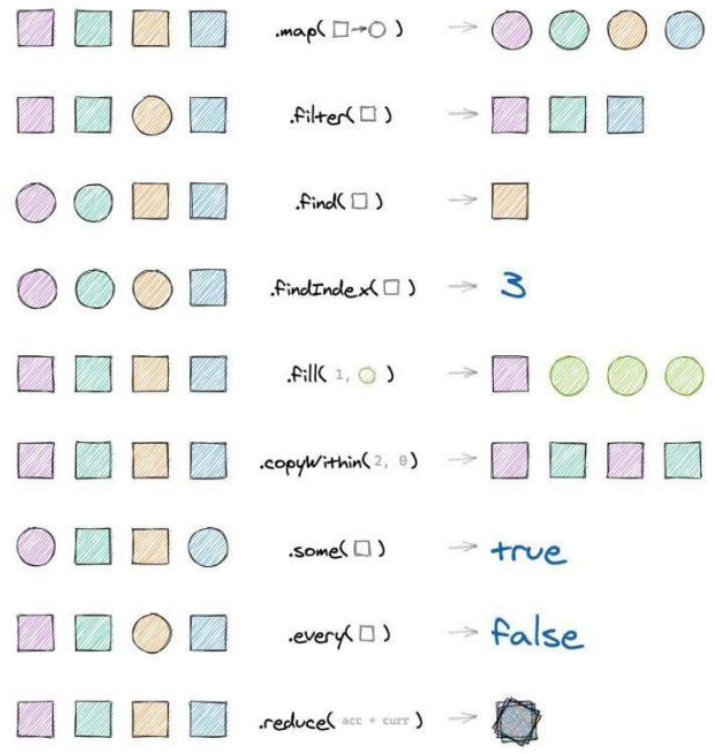
\includegraphics[width=0.5\linewidth]{images/array_cheatsheet.png}

\textcolor{red}{Achtung:} draw new!!!
\end{formula}
 
\subsection{Funktionen und funktionale Programmierung}

\begin{definition}{Funktionen}
    \begin{itemize}
        \item Funktionen sind spezielle, aufrufbare Objekte
        \item Man kann ihnen jederzeit Attribute oder Methoden hinzufügen
        \item Sie haben bereits vordefinierte Methoden
      \end{itemize}
\begin{lstlisting}[language=JavaScript, style=basesmol]
> const add = (x, y) => x + y
> add.doc = "This function adds two values"
> add(3,4)
7
> add.doc
'This function adds two values'
\end{lstlisting}
\end{definition}

\begin{concept}{Modulsystem in JavaScript}
    \begin{itemize}
        \item \texttt{import} und \texttt{export} für Module
        \item \texttt{export default} für Standardexport
        \item \texttt{import \{name\} from 'module'} für benannte Exports
        \item \texttt{import * as name from 'module'} für alle Exports
    \end{itemize}
\begin{lstlisting}[language=JavaScript, style=basesmol]
const car = {                   //car-lib.js
    brand: 'Ford',
    model: 'Fiesta'
}
module.exports = car
const car = require('./car-lib') //other js file
\end{lstlisting}
\end{concept}

\subsection{Prototypen von Objekten}

\begin{definition}{Prototypen}
    \begin{itemize}
        \item Die meisten Objekte haben ein Prototyp-Objekt.
        \item Dieses fungiert als Fallback für Attribute und Methoden.
      \end{itemize}
\begin{lstlisting}[language=JavaScript, style=basesmol, numbers=none, xleftmargin=-2pt]
>Object.getPrototypeOf(Math.max)==Function.prototype
true
>Object.getPrototypeOf([])==Array.prototype
true
>Object.getPrototypeOf(Function.prototype)==Object.prototype
true
>Object.getPrototypeOf(Array.prototype)==Object.prototype
true
\end{lstlisting}
\end{definition}

\begin{concept}{Prototypen-Kette}
    Call, apply, bind
    \begin{itemize}
        \item Weitere Argumente von call : Argumente der Funktion
        \item Weiteres Argument von apply : Array mit den Argumenten
        \item Erzeugt neue Funktion mit gebundenem this
    \end{itemize}
\begin{lstlisting}[language=JavaScript, style=basesmol]
function Employee (name, salary) {
    Person.call(this, name)
    this.salary = salary
}
Employee.prototype = new Person()
Employee.prototype.constructor = Employee
let e17 = new Employee("Mary", 7000)
console.log(e17.toString()) // Person with name 'Mary' 
console.log(e17.salary) // 7000 
\end{lstlisting}
\end{concept}

\begin{definition}{Klassen}
    \begin{itemize}
        \item Klassen sind syntaktischer Zucker für Prototypen
        \item Klassen können Attribute und Methoden enthalten
        \item Klassen können von anderen Klassen erben
    \end{itemize}
\begin{lstlisting}[language=JavaScript, style=basesmol]
class Person {
    constructor (name) {
        this.name = name
    }
    toString () {
        return `Person with name '${this.name}'
    }
}
let p35 = new Person("John")
console.log(p35.toString()) // Person with name 'John'
\end{lstlisting}
\end{definition}

\begin{code}{Vererbung}
\begin{lstlisting}[language=JavaScript, style=basesmol]
class Employee extends Person {
    constructor (name, salary) {
        super(name)
        this.salary = salary
    }
    toString () {
        return `${super.toString()} and salary ${this.salary}
    }
}
let e17 = new Employee("Mary", 7000);
console.log(e17.toString()) /* Person with name 'Mary' and salary 7000 */
console.log(e17.salary) /* 7000 */
\end{lstlisting}
\end{code}

\begin{examplecode}{Getter und Setter}
\begin{lstlisting}[language=JavaScript, style=basesmol]
class PartTimeEmployee extends Employee {
    constructor (name, salary, percentage) {
        super(name, salary)
        this.percentage = percentage
    }
    get salary100 () { return this.salary * 100 / this.percentage}
    set salary100 (amount) { this.salary = amount * this.percentage / 100 }
}
let e18 = new PartTimeEmployee("Bob", 4000, 50)
console.log(e18.salary100) /* -> 8000 */
e18.salary100 = 9000
console.log(e18.salary) /* \ 4500 */
\end{lstlisting}
\end{examplecode}


\subsubsection{Filesystem}

\begin{code}{Pfade der Datei}
Um Pfad-informationen einer Datei zu ermitteln muss man dies mit require('path') machen.
\begin{lstlisting}[language=JavaScript, style=basesmol]
const path = require('path')
const notes = '/users/bkrt/notes.txt'
path.dirname(notes) /* /users/bkrt */
path.basename(notes) /* notes.txt */
path.extname(notes) /* .txt */
path.basename(notes, path.extname(notes)) /* notes */
\end{lstlisting}
\end{code}

\begin{definition}{File API}
    Mit require('fs') wird auf die File-Api zugegriffen.
    Die File-Api bietet Funktionen zum Lesen und Schreiben von Dateien.
\end{definition}

\begin{formula}{FS Funktionen}
\begin{itemize}
    \item \texttt{fs.access}: Zugriff auf Datei oder Ordner prüfen
    \item \texttt{fs.mkdir}: Verzeichnis anlegen
    \item \texttt{fs.readdir}: Verzeichnis lesen, liefert Array von Einträgen
    \item \texttt{fs.rename}: Verzeichnis umbenennen
    \item \texttt{fs.rmdir}: Verzeichnis löschen
    \item \texttt{fs.chmod}: Berechtigungen ändern
    \item \texttt{fs.chown}: Besitzer und Gruppe ändern
    \item \texttt{fs.copyFile}: Datei kopieren
    \item \texttt{fs.link}: Besitzer und Gruppe ändern
    \item \texttt{fs.symlink}: Symbolic Link anlegen
    \item \texttt{fs.watchFile}: Datei auf Änderungen überwachen
\end{itemize}
\end{formula}

\begin{code}{Datei-Informationen}
\begin{lstlisting}[language=JavaScript, style=basesmol]
const fs = require('fs')
fs.stat('test.txt' , (err, stats) => {
    if (err) {
    console.error(err)
    return
    }
    stats.isFile() /* true */
    stats.isDirectory() /* false */
    stats.isSymbolicLink() /* false */
stats.size /* 1024000 = ca 1MB */
})
\end{lstlisting}
\end{code}

\begin{examplecode}{Dateien lesen und schreiben}
\begin{lstlisting}[language=JavaScript, style=basesmol]
const fs = require('fs')
fs.readFile('/etc/hosts',"utf8", (err, data) => {
        if (err) throw err
        console.log(data)
})

const content = 'Node was here!'
fs.writeFile('/Users/bkrt/test.txt', content, (err) => {
    if (err) {
        console.error(`Failed to write file: ${err}`)
        return
    } // file written successfully
})
\end{lstlisting}
\end{examplecode}

\subsection{Asynchrone Programmierung}

% Asynchronous Programming
\begin{concept}{Asynchrone Programmierung}\\
    JavaScript verwendet verschiedene Mechanismen für asynchrone Operationen:
    \begin{itemize}
        \item Callbacks: Traditioneller Ansatz
        \item Promises: Moderner Ansatz für strukturiertere asynchrone Operationen
        \item Async/Await: Syntaktischer Zucker für Promises
    \end{itemize}
\end{concept}

\subsubsection{Callbacks und Timers}

\begin{definition}{Callbacks}
Ein Callback ist eine Funktion, welche als Argument einer anderen Funktion übergeben wird und erst aufgerufen wird, wenn das Ereignis eingetreten ist. 
In der folgenden Abbildung wird die KlickFunktion vom Button mit der Id «Button» abonniert.
\begin{lstlisting}[language=JavaScript, style=basesmol]
document.getElementById('button').addEventListener('click', () => {
//item clicked
})
\end{lstlisting}
\end{definition}

\begin{code}{SetTimeout}
\begin{itemize}
  \item Mit setTimeout kann Code definiert werden, der zu einem späteren Zeitpunkt ausgeführt werden soll
  \item Eintrag in die Timer-Liste, auch wenn Zeit auf 0 gesetzt wird
  \item Kann mit clearTimeout entfernt werden
\end{itemize}
\begin{lstlisting}[language=JavaScript, style=basesmol]
setTimeout(() => {
    /* runs after 50 milliseconds */
}, 50)
\end{lstlisting}
\end{code}

\begin{code}{SetInterval}
\begin{itemize}
  \item Callback alle n Millisekunden in die Callback Queue eingefügt
  \item Kann mit clearInterval beendet werden
\end{itemize}
\begin{lstlisting}[language=JavaScript, style=basesmol]
const id = setInterval(() => {
// runs every 2 seconds
}, 2000)
clearInterval(id)
\end{lstlisting}
\end{code}

\begin{code}{SetImmediate}
\begin{itemize}
  \item Callback wird in die Immediate Queue eingefügt
  \item Wird nach dem aktuellen Event-Loop ausgeführt
\end{itemize}
\begin{lstlisting}[language=JavaScript, style=basesmol]
setImmediate(() => {
    console.log('immediate')
})
\end{lstlisting}
\end{code}

\subsubsection{Events und Promises}

\begin{definition}{Event-Modul (EventMitter)}
\begin{itemize}
  \item EventEmitter verwaltet Liste von Listeners zu bestimmten Events
  \item Listener für das Event können hinzugefügt oder entfernt werden
  \item Event kann ausgelöst werden $\rightarrow$ Listener werden informiert
\end{itemize}
\end{definition}

\begin{examplecode}{Listener hinzufügen}
\begin{lstlisting}[language=JavaScript, style=basesmol]
const EventEmitter = require('events')
const door = new EventEmitter()

door.on('open', () => {
    console.log('Door was opened')
})
\end{lstlisting}
\end{examplecode}

\begin{examplecode}{Event auslösen}
\begin{lstlisting}[language=JavaScript, style=basesmol]
door.on('open', (speed) => {
    console.log(`Door was opened, speed: ${speed || 'unknown'}`)
})

door.emit('open')
door.emit('open', 'slow')
\end{lstlisting}
\end{examplecode}

\begin{definition}{Promises}
Ist ein Platzhalter für einen Wert, der erst später voraussichtlich verfügbar sein wird.
Funktion mit Promise:
\begin{lstlisting}[language=JavaScript, style=basesmol]
function readFilePromise(file) {
    let promise = new Promise(function resolver(resolve, reject) {
        fs.readFile(file, "utf8", (err, data) => {
            if (err) reject(err);
            else resolve(data);
        });
    });
    return promise;
}
\end{lstlisting}
Gibt nun ein Promise-Object zurück
\end{definition}

\begin{concept}{Promise-Konstruktor erhält resolver-Funktion}

Rückgabe einer Promise: potentieller Wert kann später erfüllt oder zurückgewiesen werden
\begin{itemize}
  \item Rückgabe einer Promise: potentieller Wert
  \item kann später erfüllt oder zurückgewiesen werden
\end{itemize}
Aufruf neu:
\begin{lstlisting}[language=JavaScript, style=basesmol]
readFilePromise('/etc/hosts')
    .then(console.log)
    .catch(() => {
        console.log("Error reading file")
    })
\end{lstlisting}
\end{concept}

\begin{theorem}{Promise-Zustände}
\begin{itemize}
  \item pending: Ausgangzustand
  \item fulfilled: erfolgreich abgeschlossen
  \item rejected: ohne Erfolg abgeschlossen
  \end{itemize}
  Nur ein Zustandsübergang möglich und Zustand in Promise-Objekt gekapselt\\
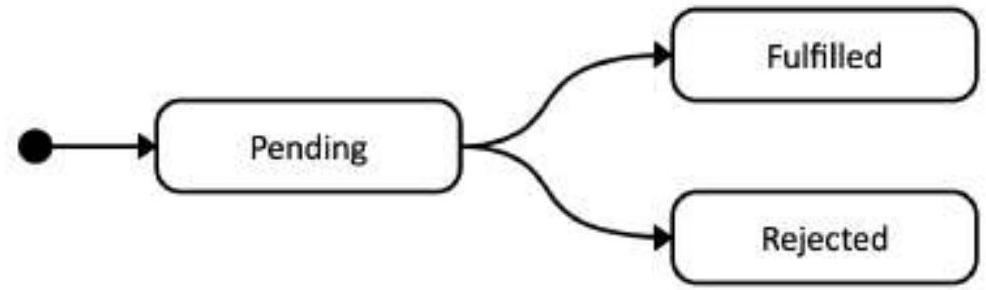
\includegraphics[width=0.8\linewidth]{images/2024_12_29_858f09cde51177c71657g-14}
\end{theorem}

\begin{corollary}{Promises Verknüpfen}
\begin{itemize}
  \item Then-Aufruf gibt selbst Promise zurück
  \item Catch-Aufruf ebenfalls, per Default erfüllt
  \item So können diese Aufrufe verkettet werden
  \item Promise, welche unmittelbar resolved wird: Promise.resolve (...)
  \item Promise, welche unmittelbar rejected wird: Promise.reject (...)
\end{itemize}
\end{corollary}

\begin{definition}{Promise.all()}
\begin{itemize}
  \item Erhält Array von Promises
  \item Erfüllt mit Array der Result, wenn alle erfüllt sind
  \item Zurückgewiesen sobald eine Promise zurückgewiesen wird
\end{itemize}
\end{definition}

\begin{definition}{Promise.race()}
\begin{itemize}
  \item Erhält Array von Promises
  \item Erfüllt sobald eine davon erfüllt ist
  \item Zurückgewiesen sobald eine davon zurückgewiesen wird
\end{itemize}
\end{definition}

\begin{code}{ASYNC/AWAIT}
\begin{lstlisting}[language=JavaScript, style=basesmol]
/* Bekanntes Beispiel */
const readHosts =() => {
    readFilePromise('/etc/hosts')
        .then(console.log)
        . catch(() => {
            console.log("Error reading file")
        })
}
/* Mit async/await */
const readHosts = async () => {
    try {
        console.log(await readFilePromise('/etc/hosts'))
    }
    catch (err) {
        console.log("Error reading file")
    }
}
\end{lstlisting}
Beispiel 2:
\begin{lstlisting}[language=JavaScript, style=basesmol]
function resolveAfter2Seconds (x) {
    return new Promise(resolve => {
        setTimeout(() => {
            resolve(x)
        }, 2000)
    })
}
async function add1(x) {
    var a = resolveAfter2Seconds(20)
    var b = resolveAfter2Seconds(30)
    return x + await a + await b
}
add1(10).then(console.log)
\end{lstlisting}
\end{code}

\begin{KR}{Promise Erstellung und Verwendung}
\begin{lstlisting}[language=JavaScript, style=basesmol]
// Promise erstellen
const myPromise = new Promise((resolve, reject) => {
    // Asynchrone Operation
    setTimeout(() => {
        if (/* erfolg */) {
            resolve(result);
        } else {
            reject(error);
        }
    }, 1000);
});

// Promise verwenden
myPromise
    .then(result => {
        // Erfolgsfall
    })
    .catch(error => {
        // Fehlerfall
    })
    .finally(() => {
        // Wird immer ausgefuhrt
    });

// Async/Await Syntax
async function myAsync() {
    try {
        const result = await myPromise;
        // Erfolgsfall
    } catch (error) {
        // Fehlerfall
    }
}
\end{lstlisting}
\end{KR}

% Modules and Node.js
\begin{concept}{Module System}
    JavaScript verwendet verschiedene Modulsysteme:
    \begin{itemize}
        \item CommonJS (Node.js): \texttt{require}/\texttt{module.exports}
        \item ES Modules: \texttt{import}/\texttt{export}
    \end{itemize}
\end{concept}

\begin{KR}{Module Import/Export}
\begin{lstlisting}[language=JavaScript, style=basesmol]
// CommonJS (Node.js)
const fs = require('fs');
module.exports = { /* ... */ };

// ES Modules
import { function1, function2 } from './module.js';
export const variable = 42;
export default class MyClass { /* ... */ }
\end{lstlisting}
\end{KR}

% Error Handling
\begin{KR}{Error Handling}
\begin{lstlisting}[language=JavaScript, style=basesmol]
try {
    // Code der Fehler werfen konnte
    throw new Error('Something went wrong');
} catch (error) {
    // Fehlerbehandlung
    console.error(error.message);
} finally {
    // Wird immer ausgefuhrt
    cleanup();
}
\end{lstlisting}
\end{KR}

\subsection{Webserver}
Die Standard-Ports von einem Webserver sind 80 und 443. Der Webserver wartet auf eine Anfrage vom Client.

\begin{definition}{Server im Internet}
\begin{itemize}
  \item Wartet auf Anfragen auf bestimmtem Port
  \item Client stellt Verbindung her und sendet Anfrage
  \item Server beantwortet Anfrage
\end{itemize}
\end{definition}

\begin{corollary}{Ports}
\begin{center}
\begin{tabular}{|l|l|}
\hline
Port & Service \\
\hline
$\mathbf{2 0}$ & FTP - Data \\
\hline
$\mathbf{2 1}$ & FTP - Control \\
\hline
$\mathbf{2 2}$ & SSH Remote Login Protocol \\
\hline
$\mathbf{2 3}$ & Telnet \\
\hline
$\mathbf{2 5}$ & Simple Mail Transfer Protocol (SMTP) \\
\hline
$\mathbf{5 3}$ & Domain Name System (DNS) \\
\hline
$\mathbf{8 0}$ & HTTP \\
\hline
$\mathbf{4 4 3}$ & HTTPs \\
\hline
\end{tabular}
\end{center}
\end{corollary}

\begin{definition}
    {File-Transfer} File Server\\
    Um Dateien auf einem File-Server auszutauschen, werden die Protokolle FTP (File Transfer Protocol) und SFTP (SSH File Transfer Protocol) verwendet.
\end{definition}

\subsubsection{HTTP}

\begin{theorem}{HTTP-Requests}
    \begin{itemize}
        \item GET: Ressource laden
        \item POST: Informationen senden
        \item PUT: Ressource anlegen, überschreiben
        \item PATCH: Ressource anpassen
        \item DELETE: Ressource löschen
    \end{itemize}
\end{theorem}

\begin{corollary}{HTTP-Response Codes}
    \begin{center}
    \begin{tabular}{|l|l|}
    \hline
    Code & Beschreibung \\
    \hline
    $\mathbf{1 x x}$ & Information (101 Switching protocols) \\
    \hline
    $\mathbf{2 x x}$ & Erfolg (200 OK) \\
    \hline
    $\mathbf{3 x x}$ & Weiterleitung (301 Moved permanently) \\
    \hline
    $\mathbf{4 x x}$ & Fehler in Anfrage (403 Forbidden, 404 Not Found) \\
    \hline
    $\mathbf{5 x x}$ & Server-Fehler (501 Not implemented) \\
    \hline
    \end{tabular}
    \end{center}
\end{corollary}

\columnbreak

\subsection{Einfacher Webserver (Node.js)}

\begin{concept}{Node.js Webserver}
\begin{lstlisting}[language=JavaScript, style=basesmol]
const {createServer} = require("http")
Let server = createServer((request, response) => {
    response.writeHead(200, {"Content-Type": "text/html"})
    response.write(`
        <h1>Hello!</h1>
        <p>You asked for <code>${request.url}</code></p>`)
    response.end()
})
server.listen(8000)
console.log("Listening! (port 8000)")|
\end{lstlisting}
\end{concept}


\begin{code}{Einfacher Webclient}
\begin{lstlisting}[language=JavaScript, style=basesmol]
const {request} = require("http")
let requestStream = request({
    hostname: "eloquentjavascript.net",
        path: "/20_node.html",
        method: "GET"
        headers: {Accept: "text/html"}
}, response => {
        console.log("Server responded with status code", response.statusCode)
})
requestStream.end()
\end{lstlisting}
\end{code}

\begin{examplecode}{Server und Client mit Streams}
\begin{lstlisting}[language=JavaScript, style=basesmol]
const {createServer} = require("http")
createServer((request, response) => {
    response.writeHead(200, {"Content-Type": "text/plain"})
        request.on("data", chunk =>
            response.write(chunk.toString().toUpperCase()))
        request.on("end" , () => response.end())
    }).listen(8000)
\end{lstlisting}

\begin{lstlisting}[language=JavaScript, style=basesmol]
const {request} = require("http")
Let rq = request({
    hostname: "localhost",
    port: 8000,
    method: "POST"
}, response => {
    response.on("data", chunk =>
    process.stdout.write(chunk.toString()));
})
rq.write("Hello server\n")
rq.write("And good bye\n")
rq.end()
\end{lstlisting}
\end{examplecode}

\begin{definition}{REST API}
\begin{itemize}
  \item REST: Representational State Transfer
  \item Zugriff auf Ressourcen über ihre Adresse (URI)
  \item Kein Zustand: jede Anfrage komplett unabhängig
  \item Kein Bezug zu vorhergehenden Anfragen
  \item Alle nötigen Informationen in Anfrage enthalten
  \item Verwenden der HTTP-Methoden: GET , PUT , POST , ...
\end{itemize}
\end{definition}

\begin{concept}{Express.js}\\
    Express.js ist ein minimales, aber flexibles Framework für Web-apps. Es hat zahlreiche Utilities und Erweiterungen. 
    Express.js basiert auf Node.js.
    $\rightarrow$ http://expressjs.com
\end{concept}


\begin{KR}{Installation}
\begin{itemize}
  \item Der Schritt npm init fragt eine Reihe von Informationen (Projektname, Version, ...) zum Projekt ab
  \item Als Entry Point ist hier index.js voreingestellt
  \item Das kann zum Beispiel in app.js geändert werden.
\end{itemize}
\begin{lstlisting}[language=JavaScript, style=basesmol]
$ mkdir myapp
$ cd myapp
$ npm init
$ npm install express --save
\end{lstlisting}
\end{KR}

\begin{code}{Beispiel: Express Server}
\begin{lstlisting}[language=JavaScript, style=basesmol]
const express = require('express')
const app = express()
const port = 3000
app.get('/', (req, res) => {
        res.send('Hello World!')
})
app.listen(port, () => {
    console.log(`Example app listening at http://localhost:${port}`)
}})
\end{lstlisting}
\end{code}

\begin{KR}{Routing}
\begin{lstlisting}[language=JavaScript, style=basesmol]
app.get('/', function (req, res) {
    res.send('Hello World!')
})
app.post('/', function (req, res) {
    res.send('Got a POST request')
})
app.put('/user', function (req, res) {
    res.send('Got a PUT request at /user')
})
app.delete('/user', function (req, res) {
    res.send('Got a DELETE request at /user')
})
\end{lstlisting}
\end{KR}






\subsection{Jasmine (Testing)}

\begin{examplecode}{Beispiel (zugehörige Tests)}
\begin{lstlisting}[language=JavaScript, style=basesmol]
/* PlayerSpec.js - Auszug */
describe("when song has been paused", function() {
    beforeEach(function() {
        player.play(song)
        player.pause()
    })
    it("should indicate that the song is currently paused", function() {
        expect(player.isPlaying).toBeFalsy()
        /* demonstrates use of 'not' with a custom matcher */
        expect(player).not.toBePlaying(song)
    })
    it("should be possible to resume", function() {
        player.resume()
        expect(player.isPlaying).toBeTruthy()
        expect(player.currentlyPlayingSong) .toEqual(song)
    })
})
\end{lstlisting}
\end{examplecode}

\begin{code}{JASMINE: MATCHER}
\begin{lstlisting}[language=JavaScript, style=basesmol]
expect([1, 2, 3]).toEqual([1, 2, 3])
expect(12).toBeTruthy()
expect("").toBeFalsy()
expect("Hello planet").not.toContain("world")
expect(null).toBeNull()
expect(8).toBeGreaterThan(5)
expect(12.34).toBeCloseTo(12.3, 1)
expect("horse_ebooks.jpg") .toMatch(/\w+.(jpg|gif|png|svg)/i)
\end{lstlisting}
\end{code}

\begin{KR}{JASMINE: TESTS DURCHFÜHREN}
\begin{lstlisting}[language=bash, style=basesmol]
$ npx jasmine
Randomized with seed 03741
Started
......
5 specs, 0 failures
Finished in 0.014 seconds
Randomized with seed 03741 
    (jasmine --random=true --seed=03741)
\end{lstlisting}
\end{KR}